%% 
%% Copyright 2007-2020 Elsevier Ltd
%% 
%% This file is part of the 'Elsarticle Bundle'.
%% ---------------------------------------------
%% 
%% It may be distributed under the conditions of the LaTeX Project Public
%% License, either version 1.2 of this license or (at your option) any
%% later version.  The latest version of this license is in
%%    http://www.latex-project.org/lppl.txt
%% and version 1.2 or later is part of all distributions of LaTeX
%% version 1999/12/01 or later.
%% 
%% The list of all files belonging to the 'Elsarticle Bundle' is
%% given in the file `manifest.txt'.
%% 

%% Template article for Elsevier's document class `elsarticle'
%% with numbered style bibliographic references
%% SP 2008/03/01
%%
%% 
%%
%% $Id: elsarticle-template-num.tex 190 2020-11-23 11:12:32Z rishi $
%%
%%
\documentclass[preprint,12pt]{elsarticle}

%% Use the option review to obtain double line spacing
%% \documentclass[authoryear,preprint,review,12pt]{elsarticle}

%% Use the options 1p,twocolumn; 3p; 3p,twocolumn; 5p; or 5p,twocolumn
%% for a journal layout:
%% \documentclass[final,1p,times]{elsarticle}
%% \documentclass[final,1p,times,twocolumn]{elsarticle}
%% \documentclass[final,3p,times]{elsarticle}
%% \documentclass[final,3p,times,twocolumn]{elsarticle}
%% \documentclass[final,5p,times]{elsarticle}
%% \documentclass[final,5p,times,twocolumn]{elsarticle}

%% For including figures, graphicx.sty has been loaded in
%% elsarticle.cls. If you prefer to use the old commands
%% please give \usepackage{epsfig}

%% The amssymb package provides various useful mathematical symbols
\usepackage{amssymb}
%% The amsthm package provides extended theorem environments
%% \usepackage{amsthm}

%% The lineno packages adds line numbers. Start line numbering with
%% \begin{linenumbers}, end it with \end{linenumbers}. Or switch it on
%% for the whole article with \linenumbers.
%% \usepackage{lineno}

\journal{Optik}

\begin{document}

\begin{frontmatter}

%% Title, authors and addresses

%% use the tnoteref command within \title for footnotes;
%% use the tnotetext command for theassociated footnote;
%% use the fnref command within \author or \address for footnotes;
%% use the fntext command for theassociated footnote;
%% use the corref command within \author for corresponding author footnotes;
%% use the cortext command for theassociated footnote;
%% use the ead command for the email address,
%% and the form \ead[url] for the home page:
%% \title{Title\tnoteref{label1}}
%% \tnotetext[label1]{}
%% \author{Name\corref{cor1}\fnref{label2}}
%% \ead{email address}
%% \ead[url]{home page}
%% \fntext[label2]{}
%% \cortext[cor1]{}
%% \affiliation{organization={},
%%             addressline={},
%%             city={},
%%             postcode={},
%%             state={},
%%             country={}}
%% \fntext[label3]{}

\title{InGaN/Si Tandem solar cell}

%% use optional labels to link authors explicitly to addresses:
%%\author[label1,label3]{}
%% \affiliation[label1]{organization={},
%%             addressline={},
%%             city={},
%%             postcode={},
%%             state={},
%%             country={}}
%%
%% \affiliation[label2]{organization={},
%%             addressline={},
%%             city={},
%%             postcode={},
%%             state={},
%%             country={}}

\author{Abdelwahab Doha\fnref{label1}}
\ead{doha@gmail.com}
\affiliation[label1]{organization={University of Bechar},
            addressline={}, 
            city={},
            postcode={08.000}, 
            state={Bechar},
            country={Algeria}}
            
\author{Benameur Amiri\fnref{label2}}
\ead{lpdsamis@gmail.com}
%% \ead[url]{home page}
%% \fntext[label2]{}
%% \cortext[cor1]{}
\affiliation[label2]{organization={Higher Normal School of Bechar},
				 addressline={},
	             city={},
	             postcode={08.000},
	             state={Bechar},
	             country={Algeria}}

\author{Abdelrahmane Belghachi\fnref{label1}}
\ead{belghachi@gmail.com}


\begin{abstract}
Optical and electrical properties of $InGaN$ alloys is being intensively studied to be combined with silicon by implementing $SiO2/Si3N4$ interlayers. Adhesion of nano-interlayer appears to reduce photonic electro-migration hurdle between InGaN and Si, in order to achieve high-efficiency solar cell. However, a relatively thick layer of $InGaN$ is difficult to grow due to the relaxation issue in material. This issue can be avoided by eboxy layer. This work, we present an $InGaN/Si$ tandem solar cell modeled using Wien2k and Solcore softwares. We have shown that 25\% of indium is needed to ensure the current matching between the top cell and the bottom cell. With feasible structural parameters, we have shown that an efficiency near to 30\% can be achieved with $InGaN/Si$ tandem cell.
\end{abstract}

%%Graphical abstract
\begin{graphicalabstract}
%\includegraphics{grabs}
\end{graphicalabstract}

%%Research highlights
\begin{highlights}
\item Research highlight 1
\item Research highlight 2
\end{highlights}

\begin{keyword}
%% keywords here, in the form: keyword \sep keyword

%% PACS codes here, in the form: \PACS code \sep code

%% MSC codes here, in the form: \MSC code \sep code
%% or \MSC[2008] code \sep code (2000 is the default)

\end{keyword}

\end{frontmatter}

%% \linenumbers

%% main text
\section{Introduction} \label{sec:intro}

III-nitride $(N)$ semiconductors, including aluminum nitride $(AlN)$, gallium nitride $(GaN)$, and indium nitride $(InN)$, are highly promising building for optoelectronics and high-power electronics \cite{strite1992gan}. the III-nitrides have wurtzite crystal structure at ambient conditions, and the direct bandgap changes from 6.2 eV of $AlN$, 3.4 eV of $GaN$, to 0.7 eV of $InN$. III-Ns are displaying large amount of commercialized optoelectronics devices, including Photodetectors \cite{pernot2000solar,chen1997schottky,munoz1997photoconductor}, light-emitting diodes (LEDs) (\cite{nakamura1993high,funato2006blue,iso2007high}, laser diodes (LDs) \cite{nakamura1998continuous}, and solar cells \cite{neufeld2008high,jani2007design,jiang2017enhanced},which are applied in energy harvesting. Compared to other semiconductors, III-Ns demonstrate a fundamental advantage of the formation of heterogeneous structures, such as quantum wells, and  quantum dots. Heterogeneous structures III-N can be manufactured through key crystal growth techniques, including molecular beam epitaxy (MBE), metal-organic chemical vapor deposition (MOCVD) and hydride vapor-phase epitaxy (HVPE) \cite{jain2000iii,yoshida1982properties,li2007influence}.Due to the inability of a single solar cell to absorb large solar spectrum photons efficiently, multijunction solar cells have been the focus of much theoretical and experimental work in the past few decades. The most successful efforts to date have focused on the use of semiconductors such as II-VI and III-V alloys to construct such cells, achieving energy conversion efficiencies of over 30\%. The $InGaN$ range band gap can be engineered from 0.7 to 3.4 eV, and this makes it suitable for a range of multijunction solar cell designs. These cells are able to use high-energy photons more efficiently than those limited to band gaps of less than 2.2 eV. These cells will also have the advantage that $Si$ is relatively cheap and abundant as well as that the $Si$ range gap of 1.1 eV is ideally suited to the lower connection of a high-efficiency two-link solar cell. Growth of $InGaN$-based opto-electronic device structures on $Si$ has been extensively investigated previously with the goal of optimizing the interface layer(s) between the $Si$ and the active layers to reduce defects in the nitride layers and to improve device performance . Hsu et al.\cite{hsu2008modeling} saw at an alloy composition of $In_{0.46}Ga_{_{0.54}}N$, the conduction band of $InGaN$ has the same energy as the valence band of $Si$, and so a $n-In_{0.46}Ga_{0.54}N/p-Si$ interface should form a low resistance Ohmic junction. Recent studies have shown that high quality $InGaN$ nanostructures can be grown directly on Si substrate \cite{arafin2013review, wang2019in0}. In this study, we have performed a detailed investigation of the optimize and performance characterization of $InGaN/Si$ tandem solar cell.
\section{Methode and modelisation} \label{sec:Methode and modelisation}

Solcore is a multi-scale, modular simulation framework for solar energy research, written in Python. Is evolved from SOL, a Fortran-based, quantum well solar cell solver developed by Nelson and Connelly \cite{book1}, uses electronic and optical parameters obtained from different sources for a consistent set of electronic and optical properties. In order to calculate and model the optical response of potential solar cell and material systems, Solcore incorporates a resource of freely available optical constant data measured by Sopra S. A. and provided by Spectra Inc.\cite{sopra2008optical}. To calculate the band structure of a material Solcore includes a modified 8-band Pikus–Bir Hamiltonian under biaxial strain, considering the coupling between the conduction, heavy hole, light hole and split-off bands. The eigenfunctions $\psi$ and eigenstates E are the solutions of the following equation, where H is the Pikus–Bir Hamiltonian:

.................................
.................................

To evaluate the realistic optical behaviour of a solar cell, and obtain the fraction of incoming light reflected, absorbed, and transmitted as a function of the wavelength of the light and the position inside the structure. it is important to consider the interaction of incident electromagnetic (EM) radiation with a succession of both absorbing and non-absorbing planar layers using the  transfer matrix method (TMM), The implementation of the TMM in Solcore uses the freely available tmm module developed by Byrnes \cite{byrnes2016multilayer}. Solcore includes four solvers to calculate the electrical properties of a single-junction device, these are: detailed balance, 2-diode equation, depletion approximation, and Poisson–drift–diffusion. To combine them into a multi-junction device, it is necessary
to consider that the individual junctions are electrically connected in series and the potential coupling of light emitted by the wider bandgap junctions into those with smaller bandgap.

\section{Resultat and Discution} \label{sec:Resultat and Discution}
The simulation begins from the thickness of the nominal layer and the refractive index calculated using the DFT theory impleted in Wien 2k software, we process this optimization in two phases: a optical simulation to get approximate total thicknesses for each junction, and then a device optimization. Using TMM simulation to calculate the photogenerated current in each layer, we get an estimate of the overall thickness of each material we will need to achieve current-matching, from a purely optical point of view the thickness of the bottom Si cell should be thick to maximize absorption, which is of course not the case for a device. Once we have good values for the layer thicknesses, we use full electrical simulation to determine the n and p thicknesses to calculate an optimize possible efficiency for the 2J device. Now that the layer thicknesses have been optimized from an optical point of view, we want to design the device.

% TODO: \usepackage{graphicx} required
\begin{figure}[h!]
	\centering
	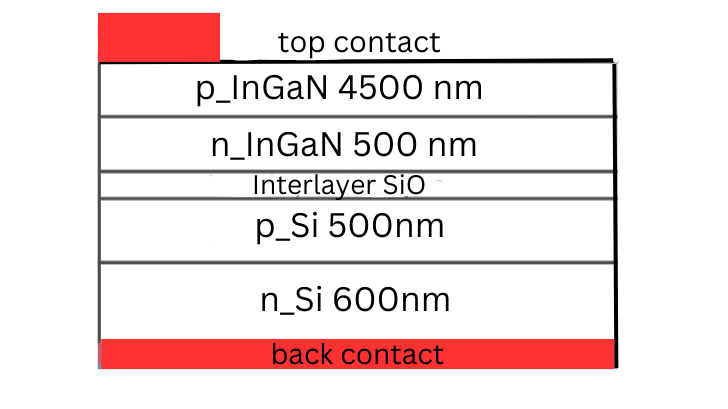
\includegraphics[width=0.7\linewidth]{Figure/structure}
	\caption{Structure of $InGaN/Si$ tandem solar cell.}
	\label{fig:structure}
\end{figure}


% TODO: \usepackage{graphicx} required
\begin{figure}[h!]
	\centering
	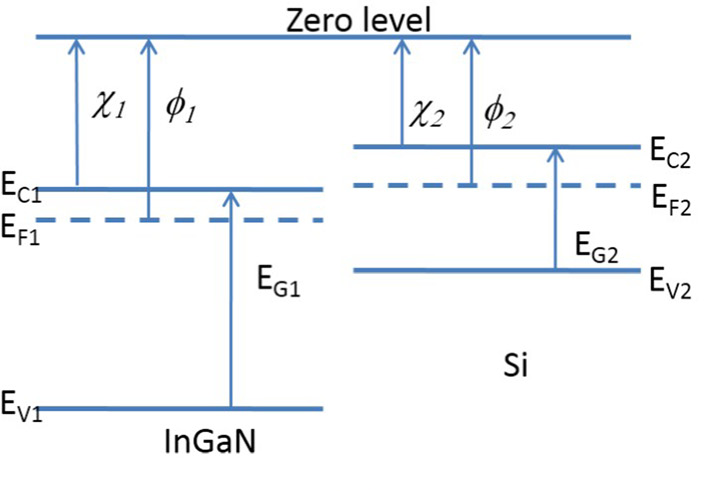
\includegraphics[width=0.7\linewidth, height=0.3\textheight]{Figure/InGaN_Si}
	\caption{Band diagrams of $InGaN$ and $Si$ before in contact}
	\label{fig:ingansi}
\end{figure}


\begin{table}[!ht]
	\centering
% ~ $Eg$~ & ~$\tau_{n}$~&~$~\tau_{p}$~&~$S_{n}$~&~ $S_{p}$ ~& ~$~\mu_{n}$~& ~$~\mu_{p}$~
	\begin{tabular}{llllll} \hline \\
		
		&~Parametre ~~~~~&~~ $CdS$~~& $Si$ & $GaN$ & $InGaN$ \\ \\ \hline \\ 
		&   &  &   & \\ \\
		&   &  &   & \\ \\
		&   &  &   & \\ \\
		&   &  &   & \\ \\
		&   &  &   & \\ \\
		&   &  &   & \\ \\
		
		&   &  &   & \\ \\
		&   &  &   & \\ \\
		&   &  &   & \\ \\
		
		&  &  &    & \\ \\
		&  &  &    & \\ \\
		&  &  &    & \\ \\ 	\hline \\ 
	\end{tabular}
	\caption{Parameters used in simulations.}
\end{table}

% TODO: \usepackage{graphicx} required
\begin{figure}[h!]
	\centering
	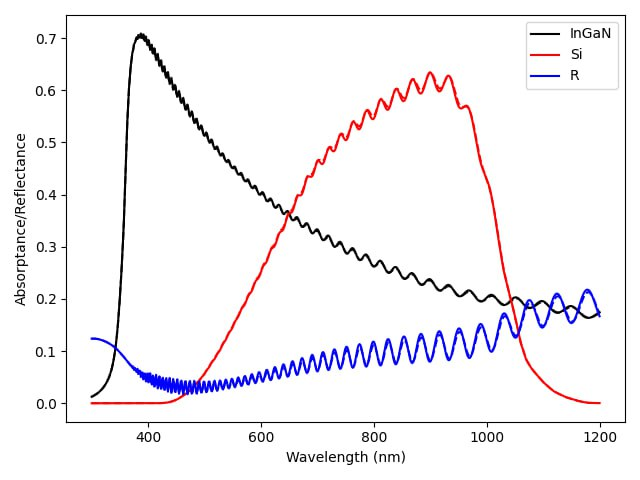
\includegraphics[width=0.7\linewidth, height=0.25\textheight]{Figure/Abs_Ref}
	\caption{}
	\label{fig:absref}
\end{figure}

\begin{figure}[h!]
	\centering
	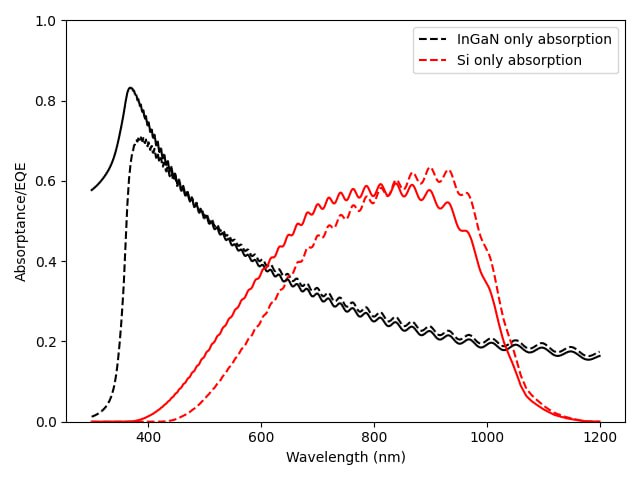
\includegraphics[width=0.7\linewidth, height=0.25\textheight]{Figure/Asorption_QE}
	\caption{}
	\label{fig:asorptionqe}
\end{figure}

\begin{figure}[h!]
	\centering
	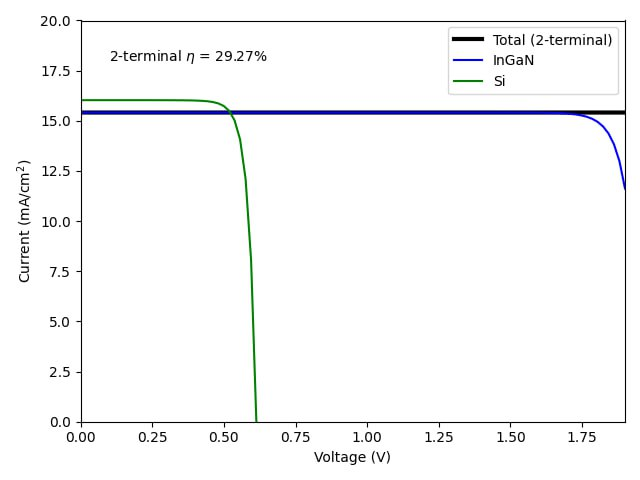
\includegraphics[width=0.7\linewidth, height=0.25\textheight]{Figure/IV}
	\caption{I-V characteristics of $In_{0.25}Ga_{0.85}N/Si$  tandem solar cell.}
	\label{fig:iv}
\end{figure}


We plot the QE and IV for the best thikness

Compare the total layer thicknesses obtained from the optical and electrical simulations:

\section{Conclusion} \label{sec:Conclusion}
Computational models based on DFT theory and K.P method can provide significant insight into photovoltaic solar cells. Calculations can be performed behaviour, through experimentally and theoric parameters such as index coefficient, band gaps and the thickness . these combines capable of modelling the optical and electrical properties of tandem solar cells. we found the optimized band-gap and the thickness of $InGaN$ top layer were 2.2 eV and 600 nm respectively acheived optimal conversion efficiency of 30\%, which is higher than that of the single junction $Si$ solar cell. 

%% The Appendices part is started with the command \appendix;
%% appendix sections are then done as normal sections
%% \appendix

%% \section{}
%% \label{}

%% If you have bibdatabase file and want bibtex to generate the
%% bibitems, please use
%%
\bibliographystyle{elsarticle-num} 
\bibliography{Ref_Doh.bib}

%% else use the following coding to input the bibitems directly in the
%% TeX file.

%%%%%%%%%%%%\begin{thebibliography}{00}

%% \bibitem{label}
%% Text of bibliographic item

%%%%%%%%%%%%%%%\bibitem{}

%%%%%%%%%%%%%%\end{thebibliography}
\end{document}
\endinput
Using SILAVCO software, we have optimized this structure
and we show, in Figure 2, that the maximal efficiency
of about 28\% is obtained with 50\% of indium and with
400-nm thickness of InGaN absorbing layer

The major loss processes of thermalization and non-absorption can be largely eliminated if the energy of the absorbed photon is marginally higher than the band gap of the cell material. This leads to the concept of the tandem cell [35][36], where multiple cells are used with different band gaps, each cell converting a narrow range of photon energies close to its band gap as shown in Figure 2.2.


The absorption coefficients for InGaN can be extracted from

The I-V characteristics of the test solar cells are summarized in Figure...

The major loss processes of thermalization and non-absorption in solar cell can be exploited if the energy of the absorbed photon is marginally higher than the band gap of the cell material. This leads to the concept of the tandem cell , where multiple cells are used with different band gaps, each cell converting a narrow range of photon energies close to its band gap [35][36]. 



InGaN has been grown either on Si or Al 2O3 using AlN, GaN and InN layers [4e6]. However, the band alignment of InGaN and Si can be exploited for the fabrication of tandem InGaN/Si heterojunction solar cells that may have power conversion efficiency higher than 30\% [7] 

%%
%% End of file `elsarticle-template-num.tex'.
